\documentclass[11pt,a4paper]{report}
\usepackage{hyperref} % for \url
\PassOptionsToPackage{hyphens}{url}\usepackage{hyperref}

% \\~\\ double new line
% images
\usepackage{graphicx} 
\usepackage{float}
\graphicspath{ {./images/} }

\usepackage{amsmath}

\usepackage[utf8]{inputenc}
\usepackage[margin=3.5cm]{geometry}

\begin{document}
\thispagestyle{empty}

\newpage

\tableofcontents
\chapter{Goals and motivation of the thesis.}
TODO change it, so it will not be copy form Michal

This graduation thesis aimed to develop a diffusion model able to generate new medical CT scans and perform quality analysis of obtained results. The motivation for the implementation of the project was solving the problem of insufficient amount of training data, required for different machine learning solutions used in medical field. The first chapter is an introduction to the study, explaining the goal and motivation of the project. Next chapter contains theoretical basis, necessary to understand the thesis: convolutional neural networks, generative and discriminative models and generative adversarial networks. In the third chapter the implementation of the project was explained, detailing the project environment, iterative course of work in the form of sprints with assigned goals and modifications of the network’s learning process as well as selected aspects of implementation. Applied modifications included: increasing the resolution of generated images, preprocessing of the training data, changes in hyperparameters of the model and in the architecture of generator and discriminator networks. In the end, obtained results are presented and analysis of their quality is conducted by comparing them to original data. The conclusions showed usefulness of GAN networks in generating medical data, however some limitations found, established the direction of further development of the project.

\chapter{Theoretical Basis}

\section{Convolution}
\section{Diffusion models}
Diffusion models are type of generative models, that aims to model disstribution of data from a given dataset. They use Markov chain, which represent sequence of steps in which small random noise is added to data and then model learns to gradually reverse diffusion steps. Diffusion model contains two compoments: forward diffusion process and reverse diffusion process.

\subsection{Forward diffusion process}
During forward diffusion process we define Markov chain with T steps, which are more and more noised samples from dataset. The result is sequence: $x_1,..., x_T$  of samples with distribution $q(x_t|x_{t-1})$:
\[ q(x_t|x_{t-1}) = N(x_t;\sqrt{1-\beta_t}x_{t-1}, \beta_tI) \]
\[ q(x_{1:T}|x_0) = \prod_{t=1}^{T}{q(x_t|x_{t-1})} \]

In each step we add small amount of Gausian noise with the variance $\beta_t$. For $T\rightarrow\infty$ $x_T$ is isotropic Gaussian distribution, however for well-chosen values of $T$ and $\beta_1,..., \beta_T$ is nearly an isotropic Gaussian distribution and is sufficient for diffusion models.

$\beta_t$ is constant increased with step $t$ according to variance schedule, linear function can be used e.g. $B_1=10^{-4}$, $B_T=0.02$ for $T=1000$. \cite{DDPM}

\begin{figure}[H]
	\centering
	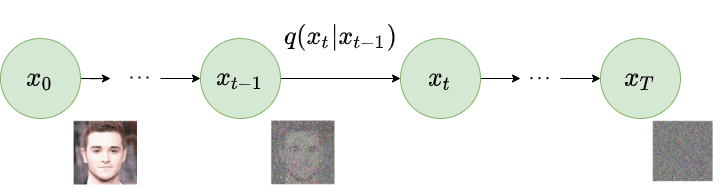
\includegraphics[width=\textwidth]{images/forward-diffusion}
    \caption{\cite{DDPM} TODO change to example from dataset (or not)}
\end{figure}

To get nth element from Markov chain we need to apply Gausian noise $n$ times, which is slow for bigget values of $n$. To improve that we can use reparameterization: let $\alpha_t = 1 - \beta_t$, $\bar{\alpha}_t = \prod_{i=1}^{t}{\alpha_i}$

\subsection{Reverse diffusion process}

\section{Attention}


\chapter{Implementation of the model}
\section{Project environment} % TODO maybe change header
\begin{itemize}
\item python 
\item pytorch
\item monai
\item hugginface diffusers 
\end{itemize}
\section{Implementation}
\url{https://github.com/Harmek59/diffusion-ct}


\addcontentsline{toc}{chapter}{\protect\numberline{}Bibliografia}
\begin{thebibliography}{99}

% TODO data of access???
\bibitem{DDPM}
\url{https://arxiv.org/pdf/2006.11239.pdf}

\bibitem{lw_diffusion}
\url{ https://lilianweng.github.io/posts/2021-07-11-diffusion-models/}
  
  
  
\end{thebibliography}
\end{document}
